%%%%%%%%%%%%%%%%%%%%%%%%%%%%%%%%%%%%%%%%%%%%%%%%%%%%%%%%%%%%%%%%%%%%%%%%%%%%%%
%
%  binary.tex
%
%  Symmetric binary fluids and Brazovskii Smetics
%
%  Edinburgh Soft Matter and Statistical Physics Group and
%  Edinburgh Parallel Computing Centre
%
%  (c) 2016 The University of Edinburgh
%
%  Contributing authors:
%  Kevin Stratford (kevin@epcc.ed.ac.uk) and I've taken material from
%  Grace Kim's                           doctoral thesis (UoE 2009)
%
%%%%%%%%%%%%%%%%%%%%%%%%%%%%%%%%%%%%%%%%%%%%%%%%%%%%%%%%%%%%%%%%%%%%%%%%%%%%%%

\section{Binary Fluids}

In this section we discuss symmetric two-component fluids, and the closely
related subject of Brazovskii smectics.\ \textit{Ludwig} was first developed
to study issues such as spinodal decomposition in binary mixtures,
so we will introduce the background in that
context (see, e.g., Swift \textit{et al.} \cite{swift1996} and Kendon
\textit{et al.}, \cite{kendon2001} for pioneering work).

Early versions of \textit{Ludwig} used, exclusively, a two lattice
Boltzmann distribution scheme to introduce the relevant dynamical update
for the binary fluid \cite{desplat2001}.
While this approach is retained in the code
for historical reasons it is often advantageous, for a number of reasons
which are set out in the following, to use a coupled lattice
Boltzmann finite-difference approach. We describe both approaches in what
follows, but reccmmend using the finite-difference approach for all current
applications. First, we consider
the common theoretical background for the two-component binary fluid.


\subsection{The Symmetric Free Energy}

\subsubsection{Thermodynamics}

For a symmetric fluid of fixed content, we define a single coarse-grained
composition
variable, or order parameter, $\phi(\mathbf{r})$. At a finer level,
one can interpret the order parameter as
$\phi(\mathbf{r}) = (n_1 - n_2)/(n_1 + n_2)$
where the $n$ are number densities of the two components. In either case,
it is an important
feature of these systems that the order parameter is conserved so that
\begin{equation}
\int \mathrm{d}\mathbf{r} (\phi - \phi_0) = 0
\end{equation}
at all times, where $\phi_0$ is the mean order parameter. In general,
if the order parameter values associated with the two components are
$\phi_1$ and $\phi_2$, then the volume fraction of the first component is
$v_1 = (\phi_2 - \phi_0)/(\phi_2 - \phi_1)$, and $v_2 = 1 - v_1$.

For a uniform
state at constant volume and temperature we can write the density of the
(Helmholtz) free energy as $V(\phi)$. In mean field theory, it is predicted
that $V(\phi)$ has uniform positive curvature at high temperature, but
becomes concave below a critical temperature $T_c$. This is illustrated
in the left panel of Fig.~\ref{figure-symmetric-schematic}.
For temperatures larger than $T_c$, there is a homogeneous state with
$\phi = 0$ everywhere, i.e., the state is fully mixed. For temperatures
below $T_c$, the free energy is minimised by creating two separate
domains, each composed of a single constituent. This results in a
phase diagram of the sort 
shown in Fig.~1 (right panel) with mixed and
separated phases bounded by a co-existance curve.

In an initially mixed system spinodal decomposition occurs when a
temperature change leaves the system below the spinodal line in the
phase diagram. This leaves the system in a globally unstable state,
and the response is initially small changes in composition
everywhere which grow smoothly in time. These small changes
ultimately create interfaces between fluid domains;
minimisation of energy then translates to minimisation of interfacial
curvature which drives the fluid domains to grow. If the quench leaves
the system between the coexistance line and the spinoal line, the
system is in a metastable state, and the response is local changes
in composition which nucleate droplets.

Note that in some real fluid mixtures, the phase diagram is inverted,
and a quench into the coexistance region is upwards in temperature.
See, e.g., Chaikin and Lubensky \cite{chaikin-lubensky} for an extended
discusion of spinodal decomposition.

Quantitatively, fluid domains together with interfaces are described
by a free energy functional with two contributions. An appropriate
choice is the Ginzburg-Landau functional, sometimes referred to as the
squared gradient model:
\begin{equation}
F[\phi]  = \int \mathrm{d}\mathbf{r} [ V(\phi) + {\textstyle\frac{1}{2}}
\kappa (\partial_\alpha \phi)^2 ] 
\end{equation}
where the $V(\phi)$ is as before and the second term penalises gradients
in the composition with parameter $\kappa > 0$. The explicit form of
$V(\phi)$ is taken here from a general Landau expansion:
\begin{equation}
V(\phi) = {\textstyle\frac{1}{2}} A \phi^2
        + {\textstyle\frac{1}{4}} B \phi^4.
\end{equation}
The minima in the
potential (cf.\ Fig.~\ref{figure-symmetric-schematic}) can then be
identified by setting
$dV / d \phi = 0$, that is, $A\phi + B\phi^3 = \phi (A + B\phi^2) = 0$.
If we take $B>0$, this condition has two cases: we denote the
solutions $\phi^\star$ in both. The first is the mixed case
which has $A > 0$ so that we
must have $\phi^\star = 0$, and the second is the separated case
which has $A < 0$ and so 
$\phi^\star = \pm (-A/B)^{1/2}$.

The combination of parameters $A,B$ and $\kappa$ also determine the
interfacial tension and the interfacial width.
The stationary values of the free energy functional can be obtained
from the Euler-Lagrange equation for $\phi$. The relevant case is
where we have a functional the density of which is written
$f(\phi, \partial_\alpha \phi)$ and the corresponding Euler-Lagrange
equation is
\begin{equation}
\frac{\partial f}{\partial \phi}
- \partial_\alpha \frac{\partial f}{\partial\, \partial_\alpha \phi} = 0.
\end{equation}

\begin{figure}[t]

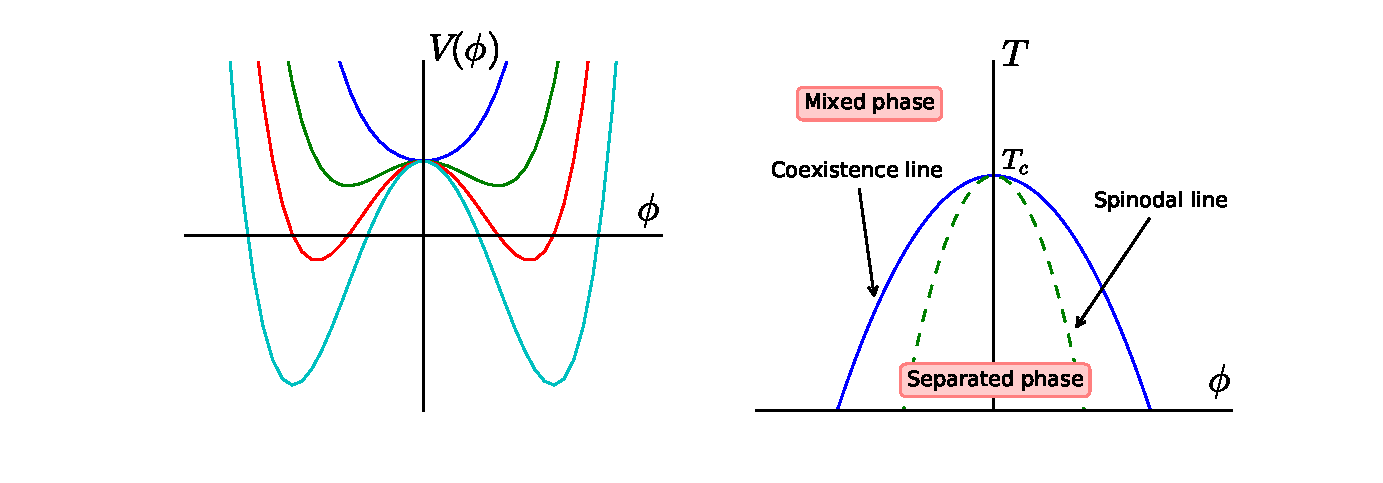
\includegraphics[width=0.9\textwidth]{figures/symmetric.eps}

\caption{Two panels showing (left) the form of the free energy density
$V(\phi)$ for the binary fluid for a number of different
temperatures. At temperatures above
the critical temperature, there is a single minimum (top curve), while
below $T_c$, two symmetric minima are present (lower curves). The related
phase diagram (right) in the temperature-composition plane shows mixed
and separated phases the boundary of which is the coexistence 
line. This (sometimes referred to as the binodal line) is the locus of
points which are the minima of $V(\phi)$ at different temperatures. The
spinodal line is formed by the locus of points which are the inflections
of $V(\phi)$.}
\label{figure-symmetric-schematic}
\end{figure}


If we consider a one-dimensional case, this is
\begin{equation}
A\phi + B\phi^3 - \kappa \frac{d^2 \phi}{dx^2} = 0.
\end{equation}
Note that the conservation of order parameter means this should be a
constrained minimisation, which can be handled by adding the
a Lagrange multiplier $\Lambda = \partial f / \partial \phi |_{\phi_0}$.
The resulting ordinary differential equation has a solution
$\phi(x) = \phi^\star \tanh(x/\xi)$ where $\xi$ is identified
as the interfacial width. It can be confirmed that this is a solution
if
\begin{equation}
\xi = (-2\kappa / A)^{1/2}.
\end{equation}
The one-dimensional case can also be used to determine the interfacial
tension, which is the excess energy associated with the interface.
If we denote the interfacial tension $\sigma$, then the excess
energy is
\begin{equation}
\sigma = \int_{-\infty}^{+\infty} \mathrm{d} x
\Big[
{\textstyle \frac{1}{2}} \kappa (d_x \phi)^2 + V(\phi) - V(\phi^\star)
\Big],
\end{equation}
which can be evaluated from the equilibrium profile with the interface
placed at the origin $\phi(x) = \phi^\star\tanh(x/\xi)$, along with a number
of standard integrals, to give
\begin{equation}
\sigma =  4\kappa\phi^{\star 2}/3\xi
 = \big(-8\kappa A^3/9B^2\big)^{1/2}.
\end{equation}
Further discussion of the practical choice of the free energy parameters,
and their
impact on interfacial width and tension is deferred until LATER.

\subsubsection{Dynamics}

In a purely diffusive regime, the time evolution of a conserved
order parameter may be expressed as the local divergence of a flux
$j_\alpha(\mathbf{r})$, that is,
$\partial_t \phi(\mathbf{r}) + \partial_\alpha j_\alpha(\mathbf{r}) = 0$.
In this picture, the system responds to small local changes in composition
by diffusion, which acts to reduce the energy. Formally, this
response of the free energy to a small change in composition is described
by the chemical potential
\begin{equation}
\mu = \frac{\delta F}{\delta \phi} = \frac{dV}{d\phi} - \kappa \partial_\alpha^2 \phi,
\end{equation}
being the functional derivative of the free energy with respect to the
order parameter. The dynamics is usually described in the context of the
model of Cahn and Hilliard \cite{cahn-hilliard-1958}, otherwise known as
Model B, where
\begin{equation}
\frac{\partial \phi}{\partial t} =
M\partial_\alpha^2 \frac{\delta F}{\delta \phi}.
\label{eq-cahn-hilliard}
\end{equation}
Here, the diffusive flux is related to the gradient of chemical potential
via $j_\alpha = -M \partial_\alpha \mu$, where $M$ is a mobilty
(taken to be uniform). 

In the presence of a fluid with velocity field $u_\alpha(\mathbf{r})$,
the full equation for the time evolution of the order parameter is
\begin{equation}
\partial_t \phi + \partial_\alpha (\phi u_\alpha + M\partial_\alpha \mu) = 0.
\label{eq-cahn-hilliard-final}
\end{equation}
This form again stresses the nature of the dynamics as a conservation law,
involving the divergence of advective fluxes $\phi u_\alpha$ and diffusive
fluxes $j_\alpha = -M\partial_\alpha \mu$. It
also admits that the mobility may be a function of position, e.g., via
$M = M(\phi)$. Equation~\ref{eq-cahn-hilliard-final} will form the basis of
the numerical solution of the binary fluid problem, coupled to the
Navier-Stokes equation.

The presence of a interface, or non-uniform composition, can lead to
thermodynamic stresses on the fluid which we denote $P_{\alpha\beta}$,
in additional to the usual viscous
stresses. The divergence of this
additional stress represents a body force density in the Navier-Stokes
equation, which is related to the chemical potential via
$f_\alpha = -\phi\partial_\alpha \mu = -\partial_\beta P_{\alpha\beta}$.
The full form of the additional stress may be related to the order
parameter by
\begin{equation}
P_{\alpha\beta} = p_0 \delta_{\alpha\beta}
  + \kappa \partial_\alpha \phi \partial_\beta \phi
\end{equation}
with isotropic contribution
\begin{equation}
p_0 = \phi \frac{dV(\phi)}{d\phi} -  V(\phi)
-\kappa\phi\partial_\alpha^2 \phi - \textstyle{\frac{1}{2}} \kappa (\partial_\alpha \phi)^2.
\end{equation}
Note that the stress $P_{\alpha\beta}$ is symmetric. At (local) equilibrium,
one expects gradients in the chemical potential to vanish,
and there will be neither diffusive fluxes ($j_\alpha = 0$) nor force on
the fluid ($f_\alpha = 0$).

\subsubsection{Surface (or wetting) free energy}

In the presence of a solid surface, the two component fluid gives
rise to the possiblity of a solid-fluid-fluid contact line. In the
symmetric case, the fluid-fluid interface will be at right angles to
a uniform flat surface. If one component wets the solid preferentially
(that is, it is energetically favourable for that component to be
in contact with the solid) the angle may move away from
90~degrees.
In general, the equilibrium contact angle $\theta$ is given by the
Young equation
\begin{equation}
\sigma_1 - \sigma_2 - \sigma \cos\theta = 0,
\end{equation}
where there are two solid-fluid surface tensions for components 1 and 2,
and the fluid-fluid interfacial tension is $\sigma$ as before.

This may be described in the free energy picture by adding a free
energy density per unit area assoicated with the surface:
\begin{equation}
f_s (\phi_s)= \textstyle{\frac{1}{2}} C \phi_s^2 + H \phi_s,
\end{equation}
where $\phi_s$ is the order parameter at the surface, and $C$ and $H$ are
constant parameters.

\subsection{Implementation}

\subsubsection{Lattice kinetic approach}

A second distribution function is introduced, denoted $g_i(\mathbf{r};t)$,
which describes the composition. The moments of this distribution, by
analogy with the hydrodynamic case with distribution
$f_i(\mathbf{r};t)$ given in
Eq.~\ref{equation-lb-f-moments}, are written
\begin{equation}
\phi(\mathbf{r};t) = \sum_i g_i (\mathbf{r};t), \quad
j_\alpha(\mathbf{r};t) = \sum_i g_i(\mathbf{r};t) c_{i\alpha}, \quad
\Phi_{\alpha\beta}(\mathbf{r};t) = \sum_i g_i(\mathbf{r};t)
c_{i\alpha}c_{i\beta}.
\end{equation}
Again, the summation is over index $i$ which counts the number of
discrete velocity components for the relevant lattice Boltzmann
model $N_{\mathrm{vel}}$. However, for the Cahn-Hilliard equation,
the only relevant physical moments are the order parameter
$\phi(\mathbf{r};t)$ and the flux $j_\alpha(\mathbf{r};t)$, so
the quantity $\Phi_{\alpha\beta}(\mathbf{r};t)$ is counted among
the kinetic modes and has no precise physical interpretation. In
contrast to the previous section, here $j_\alpha(\mathbf{r};t)$
is used to represent the total flux (advective
plus diffusive) rather than the purely diffusive flux.

The lack of direct physical interpretation for the second moment
means there are a number of possible choices at the collision
stage for the $g_i(\mathbf{r};t)$ distribution.
\begin{enumerate}
\item
Following Stratford \textit{et al.} \cite{j-stat-phys-2005}:
relax $j_\alpha$ toward the equilibrium $\phi u_\alpha$
at a rate related to the mobility and fix $\Phi_{\alpha\beta} =
\phi u_\alpha u_\beta + \mu \delta_{\alpha\beta}$.
\item
Following Kendon \textit{et al.} \cite{kendon2001}: fix both
$j_\alpha = \phi$ and
$\Phi_{} = \phi u_\alpha u_\beta + M\mu \delta_{\alpha\beta}$ so the
mobilty enters explicitly with the chemical potential.
\end{enumerate}

In both cases a reprojection is used to recover the post-collision
distributions $g_i^\star(\mathbf{r};t)$. This explicitly eliminates
kinetic modes other than $\Phi_{\alpha\beta}$. Hence
\begin{equation}
g_i = w_i \big(\phi + \phi u_\alpha c_{i\alpha}/c_s^2 +
(\mu\delta_{\alpha\beta} + \phi u_\alpha u_\beta) Q_{i\alpha\beta}/2c_s^4\big).
\end{equation}
In practice, this is not stable, and we use
\begin{equation}
g_i = \phi\delta_{i0} + w_i \big( j_\alpha c_{i\alpha} / c_s^2
+ \Phi_{\alpha\beta}Q_{i\alpha\beta} / 2c_s^4\big)
\end{equation}
where the $\delta_{i0}$ has the effect of moving most of the order
parameter into the non-propagating rest distribution $g_0$. 
This reprojection approach has the advantage that it eliminates several
spurious anisotropic terms which are introduced by a single relaxation
time approach (used by Kendon \textit{et al.}).

In the relaxation approach, the form of the relaxation for the
three components of the order parameter flux is
\begin{equation}
j_\alpha^\star =
j_\alpha - \tau_\phi^{-1} (j_\alpha - \phi u_\alpha),
\end{equation}
where $j_\alpha^\star$ is the post-collision flux and the relaxation
time $\tau_\phi$ is related to the mobility  via
\begin{equation}
\tau = {\textstyle\frac{1}{2}} + M\rho_0/\Delta t.
\end{equation}

\subsubsection{Finite difference approach}

For a number of reasons, it is advantageous to replace the lattice
kinetic approach by a conventional finite difference/finite volume
treatment of the Cahn-Hilliard equation
\begin{equation}
\partial_t \phi + \partial_\alpha ( \phi u_\alpha - M \partial_\alpha \mu) = 0.
\end{equation}
(Note that the finite difference and finite volume terminology will
be used somewhat interchanably here.) Briefly, the advantages are:
\begin{enumerate}
\item
The ambiguity in interpretation of the kinetic modes is avoided,
along with the corresponding computational overhead in memory and
memory movement.
\item
Additional features may be added to the Cahn-Hilliard equation more
easily. These might include a heterogeneous mobility $M=M(\phi)$, and
order parameter fluctuations (see below).
\end{enumerate}

\vfill
\pagebreak
